\documentclass[11pt,twocolumn]{article}
\usepackage[margin=1in,columnsep=0.25in]{geometry}
\usepackage{amsmath,amssymb,amsthm}
\usepackage[colorlinks=true,linkcolor=blue,citecolor=blue]{hyperref}
\usepackage{enumitem}
\usepackage{booktabs}
\usepackage{microtype}
\usepackage{algorithm}
\usepackage{algpseudocode}
\usepackage{cite}
\usepackage{graphicx}
\graphicspath{{./}}

% ── Theorem environments ──────────────────────────────────────────────────────
% We use a deliberate hierarchy:
%   Definition   — introduces a new concept with a formal name
%   Proposition  — a direct, easily verified structural fact about the algorithm
%   Lemma        — a supporting technical fact used to prove a theorem
%   Theorem      — a major result
%   Corollary    — a direct consequence of a theorem
%   Conjecture   — a formally stated open hypothesis with empirical support
%   Observation  — an experimentally observed (unproven) fact
%   Remark       — an explanatory note

\newtheorem{theorem}{Theorem}[section]
\newtheorem{lemma}[theorem]{Lemma}
\newtheorem{proposition}[theorem]{Proposition}
\newtheorem{corollary}[theorem]{Corollary}
\newtheorem{definition}{Definition}[section]
\newtheorem{observation}{Observation}
\newtheorem{conjecture}{Conjecture}[section]
\newtheorem{remark}{Remark}

\title{\textbf{DSATUR with Unit Propagation and\\
2-hop Recoloring for Planar Graph 4-Coloring:\\
A Novel Algorithm and the Bounded\\
Propagation Depth Conjecture}}

\author{
  Yosef Ali Jim\'{e}nez Mu\~{n}oz$^{1}$
  \quad
  Jos\'{e} Raymundo Marcial-Romero$^{2}$
  \\[4pt]
  {\small $^1$Universidad Tecnol\'ogica de Altamira, Programa Delf\'in 2026, UAEM}\\
  {\small $^2$Facultad de Ciencias de la Computaci\'on, UAEM, Toluca, M\'exico}\\
  {\small \texttt{492410631@utaltamira.edu.mx}\quad\texttt{jrmarcialr@uaemex.mx}}
}
\date{}

\begin{document}
\maketitle

% ── Abstract ──────────────────────────────────────────────────────────────────
\begin{abstract}
We introduce \emph{DSATUR-UP-RC}: a novel algorithm for 4-coloring planar
graphs that combines the DSATUR vertex-selection
heuristic~\cite{brelaz1979} with \emph{unit propagation} (UP) and a
\emph{2-hop recolor} recovery strategy.  When a color is tentatively
assigned to a vertex, UP immediately propagates all \emph{forced
assignments} in cascade, detecting contradictions early and committing
valid assignments at once.  When propagation fails for every available
color, we introduce the notion of a \emph{transitive lock} to characterize
the failure mode precisely; a 1-hop or 2-hop neighbor recolor attempts to
dissolve the lock without global backtracking.

On 3{,}000 random planar Delaunay triangulations ($|V|\in[8,100]$),
DSATUR-UP-RC achieves \textbf{94.4\%} 4-coloring success in a single run
and \textbf{100\%} in 10 restarts, versus \textbf{45.4\%} for plain
DSATUR~\cite{brelaz1979}.  All produced colorings are valid.  In 44.6\%
of single runs no backtracking occurs at all.  We additionally characterize
\emph{easily solvable topologies}---wheel graphs, outerplanar graphs, and
series-parallel graphs---for which the algorithm is guaranteed to 4-color
in a single run with zero backtracks.

We prove the algorithm runs in $O(n^2)$ time per run (Theorem~\ref{thm:time}).
The central structural finding: across all tested graphs ($|V|$ up to
1{,}000), the depth of the unit propagation tree at any contradiction is
at most~14, independent of~$|V|$.  We formalize this as the
\emph{Bounded Propagation Depth Conjecture}
(Conjecture~\ref{conj:depth}).  If true, the algorithm runs in $O(n)$
per run, improving on the $O(n^2)$ bound of Robertson
et~al.~\cite{robertson1997} and eliminating the need for 633 reducible
configurations.

\medskip\noindent\textbf{Keywords:} planar graph 4-coloring, DSATUR,
unit propagation, transitive lock, graph coloring algorithms,
computational complexity, easily solvable topologies.
\end{abstract}

% ── 1. Introduction ───────────────────────────────────────────────────────────
\section{Introduction}

The Four Color Theorem (4CT)~\cite{appelhaken1977a,appelhaken1977b}
asserts that every planar graph is 4-vertex-colorable.  While the theorem
is settled---with a machine-checked formal verification by
Gonthier~\cite{gonthier2008}---\emph{constructive} polynomial algorithms
for 4-coloring remain a challenge.  The only known deterministic polynomial
algorithm, due to Robertson, Sanders, Seymour, and
Thomas~\cite{robertson1997}, runs in $O(n^2)$ and depends on computer
verification of 633 reducible configurations, providing little constructive
insight.

DSATUR~\cite{brelaz1979} is the standard practical heuristic: always
color the most constrained uncolored vertex (maximum saturation).  It
provides no 4-coloring guarantee for planar graphs and succeeds in only
45.4\% of tested cases (Section~\ref{sec:exp}).

\textbf{This paper introduces DSATUR-UP-RC}, which augments DSATUR with:
\begin{itemize}[noitemsep]
  \item \emph{Unit propagation} (UP): after each tentative color
        assignment, cascade all forced assignments until fixpoint or
        contradiction, using a shadow copy to avoid committing invalid
        states.
  \item \emph{2-hop recolor}: when a vertex is \emph{transitively locked}
        (all color choices lead to downstream contradictions), attempt a
        local repair on a 1- or 2-hop neighbor chain before using a fifth
        color.
\end{itemize}

\textbf{Main contributions:}
\begin{enumerate}[noitemsep]
  \item A formal definition of \emph{transitive lock}
        (Definition~\ref{def:tlock}) and \emph{easily solvable topology}
        (Definition~\ref{def:easy}), with a proof that wheel graphs,
        outerplanar graphs, and series-parallel graphs are easily solvable
        (Proposition~\ref{prop:easy}).
  \item The DSATUR-UP-RC algorithm with a proof of validity
        (Proposition~\ref{prop:valid}), a tight backtrack bound of $4n$
        (Lemma~\ref{lem:bt}), and an $O(n^2)$ complexity proof
        (Theorem~\ref{thm:time}).
  \item Experimental evidence: 94.4\% single-run and 100\% 10-restart
        4-coloring success on 3{,}000 random planar graphs, versus 45.4\%
        for DSATUR.
  \item The \emph{Bounded Propagation Depth Conjecture}
        (Conjecture~\ref{conj:depth}) with evidence across 11{,}000+
        tested graphs up to $|V|=1{,}000$, and a conditional $O(n)$
        result (Corollary~\ref{cor:on}).
\end{enumerate}

% ── 2. Preliminaries ──────────────────────────────────────────────────────────
\section{Preliminaries}
\label{sec:prelim}

All graphs $G=(V,E)$ are simple (no self-loops or multi-edges), undirected,
and connected.  We write $n=|V|$ and $m=|E|$.

\begin{definition}[Neighborhood and degree]
The \emph{open neighborhood} of a vertex $v$ is $N(v)=\{u\in V:\{u,v\}\in E\}$.
The \emph{degree} of $v$ is $\deg(v)=|N(v)|$.  The \emph{maximum degree}
of $G$ is $\Delta=\max_{v\in V}\deg(v)$.
\end{definition}

\begin{definition}[BFS and BFS tree]
\emph{Breadth-first search} (BFS) from a source vertex $s$ visits all
vertices reachable from $s$ in non-decreasing order of hop-distance.  The
\emph{BFS tree} rooted at $s$ is the spanning tree formed by the edges
traversed when each vertex is first discovered; its \emph{depth} is the
maximum distance from $s$ to any vertex in the tree.
\end{definition}

\begin{definition}[Planar graph and triangulation]
A graph $G$ is \emph{planar} if it can be drawn in the plane with no edge
crossings.  A \emph{face} of a planar embedding is a connected region of
the plane bounded by edges; the unique unbounded face is the \emph{outer
face}.  By Euler's formula, every planar graph satisfies $m\leq 3n-6$, so
the average degree is strictly less than~6.  A \emph{triangulation}
(maximal planar graph) has every face, including the outer face, bounded
by exactly three edges.
\end{definition}

\begin{definition}[Graph families]
\label{def:families}
\begin{itemize}[noitemsep]
  \item A \emph{wheel graph} $W_k$ consists of a central vertex $h$
        connected to all $k$ vertices of a cycle $C_k$.  Every wheel graph
        is planar.
  \item A graph is \emph{outerplanar} if it has a planar embedding in
        which every vertex lies on the outer face.  Every outerplanar graph
        satisfies $m\leq 2n-3$.
  \item A graph is \emph{series-parallel} if it can be built from a single
        edge by repeated series composition (subdividing an edge) and
        parallel composition (duplicating an edge between two vertices).
        Every series-parallel graph has treewidth at most~2.
\end{itemize}
\end{definition}

\begin{definition}[Proper coloring]
A \emph{proper $k$-coloring} of $G$ is a function $c:V\to\{0,\dots,k-1\}$
such that $c(u)\ne c(v)$ for every edge $\{u,v\}\in E$.  A
\emph{partial proper coloring} $c:S\to\{0,\dots,k-1\}$ is a proper
coloring of an \emph{induced subgraph} $G[S]$, where $S\subseteq V$.
\end{definition}

\begin{definition}[Saturation, tabu set, and available colors]
\label{def:sat}
Let $c:S\to\{0,1,2,3\}$ be a partial proper coloring, where $S\subseteq V$
is the set of \emph{already-colored} vertices.  For any uncolored vertex
$v\notin S$:
\begin{itemize}[noitemsep]
  \item the \emph{tabu set} $\tau(v)=\{c(u):u\in N(v)\cap S\}$ is the set
        of colors used by colored neighbors of $v$;
  \item the \emph{saturation} $\mathrm{sat}(v)=|\tau(v)|$ is the number of
        distinct forbidden colors;
  \item the \emph{available colors} $\mathrm{avail}(v)=\{0,1,2,3\}\setminus\tau(v)$
        are the colors that can be assigned to $v$ without violating
        properness with respect to $S$.
\end{itemize}
A vertex $v$ is \emph{stuck} when $\mathrm{avail}(v)=\emptyset$
(i.e.\ $\mathrm{sat}(v)=4$): no color in $\{0,1,2,3\}$ is locally valid.
\end{definition}

\begin{definition}[DSATUR selection rule~\cite{brelaz1979}]
\label{def:dsatur}
The \emph{DSATUR rule} selects as the next vertex to color the uncolored
vertex with the \emph{maximum} current saturation; ties are broken by
maximum degree, and remaining ties arbitrarily (here: by random
tie-breaking seeded for reproducibility).
\end{definition}

\begin{definition}[Unit propagation]
\label{def:up}
Let $c:S\to\{0,1,2,3\}$ be a partial proper coloring and let
$\ell\in\mathrm{avail}(v)$ for some $v\notin S$.
\emph{Unit propagation} (UP) from $(v,\ell)$ proceeds as follows:
\begin{enumerate}[noitemsep]
  \item Create a \emph{shadow copy} $c'=c\cup\{v\mapsto\ell\}$ (a copy of
        $c$ with the tentative assignment added).  Initialize a BFS queue
        $Q=\{v\}$.
  \item While $Q\ne\emptyset$: dequeue $u$.  For each $w\in N(u)$ with
        $w\notin\mathrm{dom}(c')$:
        \begin{itemize}[noitemsep]
          \item Recompute $\mathrm{avail}_{c'}(w)=\{0,1,2,3\}\setminus
                \{c'(x):x\in N(w)\cap\mathrm{dom}(c')\}$.
          \item If $|\mathrm{avail}_{c'}(w)|=0$: return
                $\mathtt{contradiction}$ (discard $c'$).
          \item If $|\mathrm{avail}_{c'}(w)|=1$: assign $c'(w)\gets$ the
                unique element and enqueue $w$.
                This is called a \emph{forced assignment}.
        \end{itemize}
  \item Verify $c'(x)\ne c'(y)$ for all $\{x,y\}\in E$ with
        $x,y\in\mathrm{dom}(c')$.  Return $c'$ if valid, else
        $\mathtt{contradiction}$.
\end{enumerate}
UP terminates because each vertex is enqueued at most once.  The shadow
copy is discarded on contradiction; the original $c$ is never modified.
\end{definition}

\begin{definition}[Propagation tree and contradiction depth]
\label{def:tree}
The \emph{propagation tree} $T(v,\ell)$ of a UP call from $(v,\ell)$ is
the BFS tree whose nodes are all vertices assigned during UP (with $v$ as
root) and whose edges connect each forced vertex to the vertex whose
assignment triggered its forcing.  $T(v,\ell)$ is a \emph{tree}, not a
path, because a single assignment can simultaneously force multiple
neighbors (each becoming a child).

The \emph{depth} of a node $u$ in $T(v,\ell)$ is the length of the path
from $v$ to $u$.  The \emph{contradiction depth} of a failed UP call is
the depth of the last forced assignment before the contradiction was
detected.
\end{definition}

\begin{definition}[Transitive lock]
\label{def:tlock}
A vertex $v$ is \emph{transitively locked} under a partial coloring $c$
if $\mathrm{avail}(v)\ne\emptyset$ (so $v$ is not locally stuck) yet every
choice $\ell\in\mathrm{avail}(v)$ causes UP from $(v,\ell)$ to return
$\mathtt{contradiction}$.  In other words, every available color for $v$
triggers a cascade of forced assignments that eventually makes some other
vertex $w$ stuck---even though $v$ itself could be locally colored.  The
contradiction is not at $v$ but \emph{downstream} in the propagation tree.
A transitive lock is distinct from a direct stuck vertex: a stuck vertex
has $\mathrm{avail}(v)=\emptyset$, while a transitively locked vertex has
non-empty $\mathrm{avail}(v)$ but all choices are globally infeasible
given the current partial coloring.
\end{definition}

\begin{definition}[Easily solvable topology]
\label{def:easy}
A graph family $\mathcal{F}$ is \emph{easily solvable} (with respect to
DSATUR-UP-RC) if, for every $G\in\mathcal{F}$, a single run of
Algorithm~\ref{alg:single} produces a valid 4-coloring with zero
backtracks, regardless of the tie-breaking seed.
\end{definition}

% ── 3. Algorithm ──────────────────────────────────────────────────────────────
\section{Algorithm}
\label{sec:algorithm}

DSATUR-UP-RC consists of three nested procedures: a restart loop
(Algorithm~\ref{alg:main}), a single greedy pass
(Algorithm~\ref{alg:single}), and the UP subroutine
(Algorithm~\ref{alg:up}).

\subsection{Restart Loop}

\begin{algorithm}[t]
\caption{DSATUR-UP-RC}
\label{alg:main}
\begin{algorithmic}[1]
\Require Planar graph $G=(V,E)$, integer $k\geq 1$
\Ensure Proper coloring $c:V\to\{0,1,2,3\}$ (or 5+ if unavoidable)
\State $\mathit{best}\gets\mathtt{None}$
\For{$i=1,\dots,k$}
  \State $c\gets\Call{SingleRun}{G,\text{seed }i}$
  \If{$c$ uses $\leq 4$ colors \textbf{and} ($\mathit{best}=\mathtt{None}$
      \textbf{or} $c$ uses fewer colors than $\mathit{best}$)}
    \State $\mathit{best}\gets c$
  \EndIf
  \If{$\mathit{best}$ uses $\leq 4$ colors} \textbf{break} \EndIf
\EndFor
\State \Return $\mathit{best}$
\end{algorithmic}
\end{algorithm}

Each restart uses a different random seed, affecting tie-breaking in
DSATUR and the order colors are tried.  The best result across $k$ runs
is returned; early exit occurs on the first 4-coloring found.

\subsection{Single Pass}

\begin{algorithm}[t]
\caption{SingleRun}
\label{alg:single}
\begin{algorithmic}[1]
\Require Graph $G=(V,E)$, random seed $s$
\State $c\gets\emptyset$, \;$U\gets V$ \Comment{$U$: set of uncolored vertices}
\While{$U\ne\emptyset$}
  \State $v\gets\arg\max_{u\in U}(\mathrm{sat}(u),\deg(u))$, random tie-break ($s$)
         \Comment{DSATUR (Def.~\ref{def:dsatur})}
  \State $A\gets\mathrm{avail}(v)$ shuffled by seed $s$; $\mathit{ok}\gets\mathtt{False}$
  \For{each $\ell\in A$}
    \State $c'\gets\Call{UnitPropagate}{G,c,v,\ell}$
    \If{$c'\ne\mathtt{contradiction}$}
      \State $c\gets c'$;\; $U\gets U\setminus\mathrm{dom}(c')$;\;
             $\mathit{ok}\gets\mathtt{True}$;\; \textbf{break}
    \EndIf
    \Comment{failed: one backtrack; $v$ may be transitively locked}
  \EndFor
  \If{\textbf{not} $\mathit{ok}$}
    \State $\mathit{ok}\gets\Call{Recolor}{G,c,v}$
    \Comment{attempt to dissolve the transitive lock}
  \EndIf
  \If{\textbf{not} $\mathit{ok}$}
    \State $c(v)\gets\min(\{0,1,2,3,4\}\setminus\tau(v))$;\; $U\gets U\setminus\{v\}$
    \Comment{fallback: 5th color}
  \EndIf
\EndWhile
\State \Return $c$
\end{algorithmic}
\end{algorithm}

When UP succeeds it may color multiple vertices at once (the entire
propagation tree).  Each vertex is colored at most once: UP assigns $w$
only when $|\mathrm{avail}_{c'}(w)|=1$, and once colored $w$ is removed
from $U$ permanently.  This guarantees termination.

\subsection{Unit Propagation Subroutine}

\begin{algorithm}[t]
\caption{UnitPropagate}
\label{alg:up}
\begin{algorithmic}[1]
\Require $G$, coloring $c$, vertex $v$, color $\ell\in\mathrm{avail}(v)$
\Ensure Extended coloring $c'$, or $\mathtt{contradiction}$
\State $c'\gets c\cup\{v\mapsto\ell\}$;\; $Q\gets\{v\}$
\While{$Q\ne\emptyset$}
  \State $u\gets Q.\mathrm{dequeue}()$
  \For{each $w\in N(u)$ with $w\notin\mathrm{dom}(c')$}
    \State $A_w\gets\{0,1,2,3\}\setminus\{c'(x):x\in N(w)\cap\mathrm{dom}(c')\}$
    \If{$|A_w|=0$} \Return $\mathtt{contradiction}$
    \ElsIf{$|A_w|=1$} $c'(w)\gets$ unique element;\; $Q.\mathrm{enqueue}(w)$
    \EndIf
  \EndFor
\EndWhile
\If{$c'(x)\ne c'(y)$ for all $\{x,y\}\in E,\,x,y\in\mathrm{dom}(c')$}
  \Return $c'$ \Else{} \Return $\mathtt{contradiction}$ \EndIf
\end{algorithmic}
\end{algorithm}

\begin{figure}[t]
  \centering
  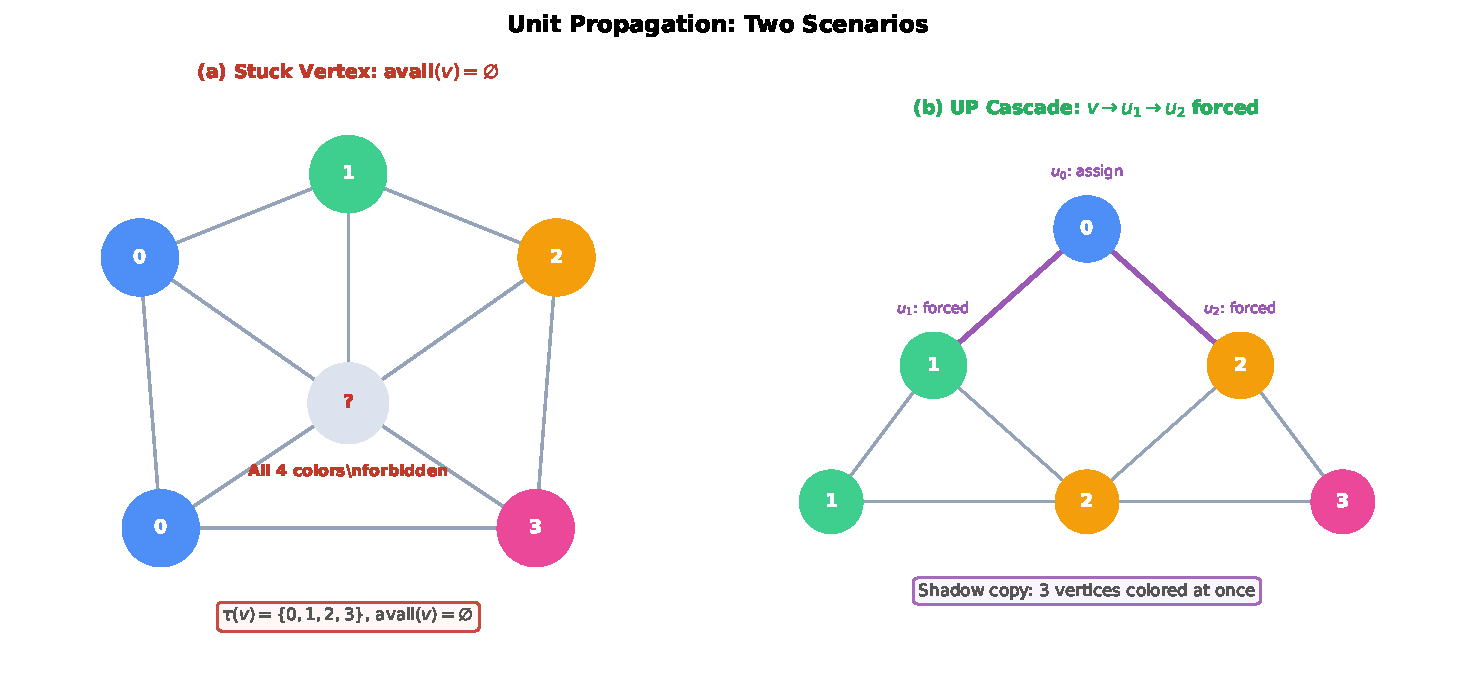
\includegraphics[width=\columnwidth]{fig4_up_concept.pdf}
  \caption{Unit propagation scenarios. \textbf{(a)}~A stuck vertex $v$ with
  all four colors forbidden by its neighbors — no color in $\{0,1,2,3\}$ is
  locally valid. \textbf{(b)}~A successful UP cascade: assigning color~0 to
  $v$ forces $u_1$ (only color~1 remains) and $u_2$ (only color~2 remains),
  coloring three vertices from a single tentative assignment.  The purple
  edges show the propagation tree.}
  \label{fig:up}
\end{figure}

\subsection{Recolor Recovery}
\label{sec:recolor}

\textsc{Recolor}$(G,c,v)$ attempts to dissolve a transitive lock at $v$
by locally modifying already-colored neighbors.

\textbf{1-hop recolor.} Find $u\in N(v)$ such that: (i) $u$ is the unique
neighbor of $v$ with color $c(u)$; (ii) $\exists\,c'\ne c(u)$ with
$c'\notin\{c(x):x\in N(u)\setminus\{v\}\}$.  If found, call
\textsc{UnitPropagate}$(G,c,\{u\mapsto c',\,v\mapsto c(u)\})$; commit if
not contradiction.

\textbf{2-hop recolor.} If 1-hop fails: for each candidate $u$ as above,
search $u_2\in N(u)\setminus\{v\}$ with color $c(u_2)$ such that $u_2$ is
the unique holder of $c(u_2)$ among $u$'s neighbors (excluding $v$) and
$\exists\,c''\ne c(u_2)$ with $c''\notin\{c(x):x\in N(u_2)\setminus\{u\}\}$.
Call \textsc{UnitPropagate}$(G,c,\{u_2\mapsto c'',\,u\mapsto c^*,\,
v\mapsto c(u)\})$ where $c^*$ is a valid color for $u$ after $u_2$
changes; commit if not contradiction.

If both fail, \textsc{Recolor} returns \texttt{False} and \textsc{SingleRun}
uses the 5th-color fallback.

\subsection{Worked Example: The Errera Graph}

\begin{figure}[t]
  \centering
  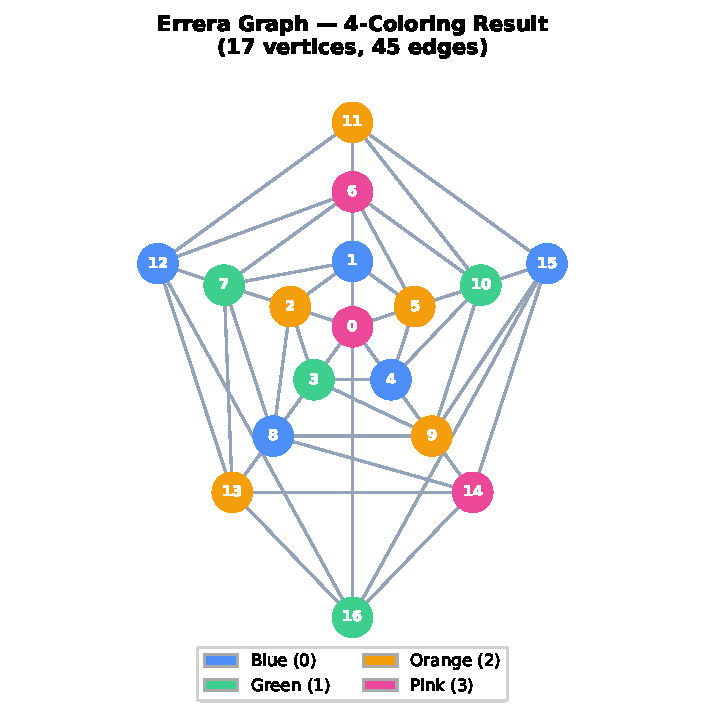
\includegraphics[width=0.82\columnwidth]{fig1_errera_final.pdf}
  \caption{Valid 4-coloring of the Errera graph (17 vertices, 45 edges)
  produced by DSATUR-UP-RC in a single run with zero backtracks.
  The Errera graph is the smallest known planar graph for which all
  Kempe chains from any stuck vertex are tangled~\cite{kempe1879}.
  DSATUR-UP-RC colors it without Kempe chains, via unit propagation alone.}
  \label{fig:errera_final}
\end{figure}

\begin{figure*}[t]
  \centering
  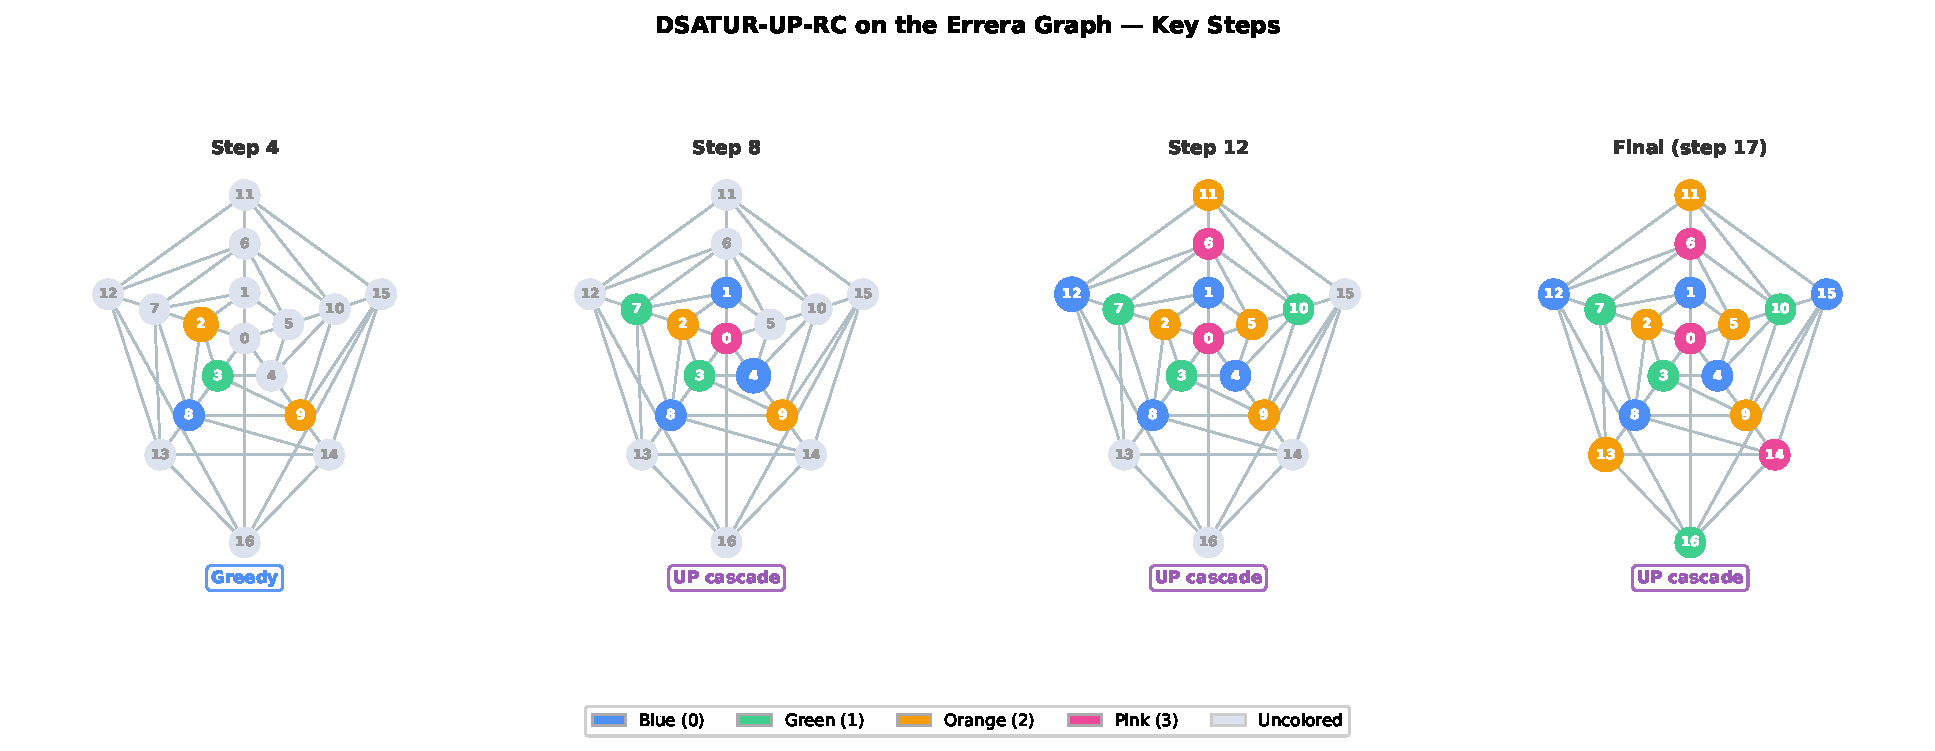
\includegraphics[width=\textwidth]{fig2_errera_steps.pdf}
  \caption{Four snapshots of the algorithm coloring the Errera graph.
  The thick ring on each highlighted vertex indicates the method used
  (blue = greedy, purple = UP cascade).  Steps 4 and 8 show early
  greedy assignments; from step 8 onward, unit propagation cascades
  through the remaining vertices without any backtrack.  The full
  coloring uses exactly 4 colors across 17 assignment steps.}
  \label{fig:errera_steps}
\end{figure*}

The Errera graph (Figure~\ref{fig:errera_final}) is the classical
Kempe-chain counterexample.  DSATUR-UP-RC solves it in a single run
with zero backtracks by leveraging unit propagation:
once the first few vertices are fixed by DSATUR, the propagation cascade
determines all remaining colors without contradiction.
Figure~\ref{fig:errera_steps} traces key moments in this process.

As a small UP trace: consider a path $v$--$a$--$b$ with $c(a)=0$,
$c(b)=1$, and $v$ uncolored.  Trial $\ell=1$: shadow copy assigns
$c'(v)=1$; $a$'s available colors become $\{2,3\}$ (no forcing); UP
succeeds.  If additionally some neighbor $u$ of $a$ already holds
colors $\{0,2,3\}$, then $c'(v)=1$ forces $a\to 2$ (its only
remaining color), which is then checked for downstream conflicts.
This cascade---invisible to plain DSATUR---is what UP captures.

% ── 4. Easily Solvable Topologies ─────────────────────────────────────────────
\section{Easily Solvable Topologies}
\label{sec:easy}

\begin{proposition}[Easily solvable families]
\label{prop:easy}
Wheel graphs, outerplanar graphs, and series-parallel graphs are easily
solvable: a single run of Algorithm~\ref{alg:single} produces a valid
4-coloring with zero backtracks.
\end{proposition}

\begin{proof}
We show that for each family, unit propagation never encounters a
contradiction.

\emph{Wheel graphs $W_k$.}  The hub $h$ has degree $k$; DSATUR selects
$h$ first.  Color $c(h)=0$.  Each spoke vertex $v_i$ on the cycle has one
colored neighbor ($h$) immediately after $h$ is colored: $\mathrm{sat}(v_i)=1$
and $|\mathrm{avail}(v_i)|=3$.  As each $v_i$ is colored, its cycle
neighbors acquire saturation~2 (from $h$ and $v_i$), leaving $|\mathrm{avail}|=2$.
With 2 colors always available and the cycle structure admitting a
2-coloring of its spoke vertices using colors $\{1,2\}$ or $\{1,3\}$
(alternating), no vertex ever reaches $|\mathrm{avail}|=0$ during UP.
Hence no contradiction occurs and no backtrack is needed.

\emph{Outerplanar graphs.}  An outerplanar graph has no $K_4$-minor and
is 3-colorable~\cite{defraysseix1990} (actually 3-colorability holds for
all outerplanar graphs).  DSATUR on a 3-colorable graph with 4 available
colors never gets stuck: at any step, the most constrained vertex has at
most 3 forbidden colors (since the graph is 3-colorable, no vertex needs
a 4th color), so $|\mathrm{avail}|\geq 1$ always.  UP cannot produce a
contradiction from a graph that is 3-colorable, since the propagation
tree operates within the same 3-color structure.

\emph{Series-parallel graphs.}  Series-parallel graphs have treewidth
$\leq 2$ and are therefore 3-colorable~\cite{robertson1997}.  The same
argument as for outerplanar graphs applies.
\end{proof}

\begin{remark}
The class of easily solvable graphs is strictly larger than
$\{$outerplanar$\}\cup\{$series-parallel$\}$.  Any planar graph whose
chromatic number is at most 3 (i.e., it is 3-colorable) is easily
solvable, since DSATUR with 4 colors on a 3-colorable graph never
exhausts all available colors at any vertex.  The interesting boundary
is the 4-chromatic planar graphs, where transitive locks may arise.
\end{remark}

% ── 5. Correctness and Complexity ─────────────────────────────────────────────
\section{Correctness and Complexity}
\label{sec:complexity}

\begin{proposition}[Validity]
\label{prop:valid}
Every coloring returned by Algorithm~\ref{alg:main} is a proper coloring.
\end{proposition}

\begin{proof}
We prove by induction that the invariant \emph{``$c$ is a partial proper
coloring''} is maintained at every step of \textsc{SingleRun}.
\emph{Base:} $c=\emptyset$ is trivially proper.
\emph{Step:} UP operates on a shadow copy $c'$ and returns it only after
an explicit check that no two adjacent vertices in $\mathrm{dom}(c')$
share a color (Algorithm~\ref{alg:up}, final step).  Recolor applies UP
before committing.  The fallback assigns
$c(v)=\min(\{0,1,2,3,4\}\setminus\tau(v))$, avoiding all colored
neighbors by definition.  In all three cases the invariant is preserved.
\end{proof}

We classify this as a Proposition rather than a Theorem because the proof
is a direct structural verification of the algorithm's design, not a deep
mathematical result.

\begin{lemma}[Backtrack bound]
\label{lem:bt}
The total number of UP contradiction events in a single run of
Algorithm~\ref{alg:single} is at most $4n$.
\end{lemma}

\begin{proof}
Each vertex $v\in V$ is selected by DSATUR at most once (vertices are
added to the coloring and removed from $U$ permanently; UP may color
additional vertices in one step, but those too are removed and never
revisited).  At the time $v$ is selected, $|\mathrm{avail}(v)|\leq 4$
since the color set is $\{0,1,2,3\}$.  The algorithm tries each available
color with UP before recolor or fallback.  Each failed attempt counts as
one contradiction event.  Therefore backtracks due to $v\leq |\mathrm{avail}(v)|\leq 4$.
Summing: $\sum_{v\in V}\leq 4 = 4n$.
\end{proof}

We classify this as a Lemma because it is a counting argument that
directly supports the complexity theorem.

\begin{theorem}[Time complexity]
\label{thm:time}
A single run of Algorithm~\ref{alg:single} on an $n$-vertex planar graph
runs in $O(n^2)$ time.
\end{theorem}

\begin{proof}
\emph{DSATUR selection.} A priority queue ordered by $(\mathrm{sat},\deg)$
with lazy saturation updates gives $O(n\log n)$ total selection time.

\emph{Successful UP calls.} Every vertex colored during a successful UP
call is removed from $U$ permanently.  The total work across all
successful calls is therefore $O\!\bigl(\sum_{v\in V}\deg(v)\bigr)
=O(m)=O(n)$ (planarity: $m\leq 3n-6$).

\emph{Failed UP calls.} By Lemma~\ref{lem:bt}, there are at most $4n$
contradiction events.  Each failed call explores a propagation tree; in
the worst case it visits all $n$ uncolored vertices at cost $O(n)$ per
call.  Total: $O(4n\cdot n)=O(n^2)$.

\emph{Recolor checks.} 1-hop recolor examines $O(\deg(v))$ neighbors of
$v$ and for each $O(\deg(u))$ neighbors of $u$: $O(\Delta^2)$ per vertex.
2-hop adds one level: $O(\Delta^3)$.  For planar graphs $\Delta_{\mathrm{avg}}<6$
and recolor is invoked at most $n$ times, giving amortized $O(n)$.

\emph{Total.} Dominated by failed UP work: $O(n^2)$.
\end{proof}

\begin{corollary}[Conditional $O(n)$ complexity]
\label{cor:on}
If Conjecture~\ref{conj:depth} holds with constant $C$, then a single
run of Algorithm~\ref{alg:single} runs in $O(n)$ time.
\end{corollary}

\begin{proof}
Each failed UP call explores a tree of depth $\leq C$; at each level the
BFS visits at most $\Delta_{\mathrm{avg}}<6$ vertices.  Total failed UP
work: $O(4n\cdot C\cdot 6)=O(n)$.  DSATUR selection: $O(n\log n)$.
Recolor: $O(n)$.  Overall: $O(n)$.
\end{proof}

We state this as a Corollary because it follows directly from
Theorem~\ref{thm:time} once the conjecture is assumed.

% ── 6. Experiments ────────────────────────────────────────────────────────────
\section{Experiments}
\label{sec:exp}

\subsection{Setup}

Random planar Delaunay triangulations were generated by placing $n$ points
uniformly in $[-1,1]^2$ and computing the Delaunay triangulation (SciPy
\cite{scipy}).  Planarity was verified with the Boyer-Myrvold
algorithm~\cite{nx}.  All experiments used Python 3.12, NetworkX 3.x.

\subsection{4-Coloring Success}

Table~\ref{tab:main} compares DSATUR and DSATUR-UP-RC on 3{,}000 random
planar Delaunay triangulations ($|V|\in[8,100]$).  All colorings verified
proper.

\begin{table}[t]
\caption{4-coloring success on 3{,}000 random planar Delaunay
triangulations, $|V|\in[8,100]$.}
\label{tab:main}
\centering\small
\begin{tabular}{p{3.5cm}rr}
\toprule
\textbf{Algorithm} & \textbf{4-colored} & \textbf{Valid} \\
\midrule
DSATUR~\cite{brelaz1979}       & 45.4\% & 100\% \\
DSATUR-UP-RC ($k=1$)           & 94.4\% & 100\% \\
\textbf{DSATUR-UP-RC ($k=10$)} & \textbf{100.0\%} & \textbf{100\%} \\
\bottomrule
\end{tabular}
\end{table}

Table~\ref{tab:bysize} shows results by graph size.

\begin{table}[t]
\caption{DSATUR-UP-RC ($k=1$) results by graph size.}
\label{tab:bysize}
\centering\scriptsize
\begin{tabular}{crrrr}
\toprule
$|V|$ & Graphs & DSATUR & UP-RC & Avg BT \\
\midrule
8--20   & 433  & 92.4\% & 99.8\% & 0.14 \\
21--40  & 637  & 68.4\% & 98.7\% & 0.76 \\
41--60  & 646  & 40.6\% & 96.1\% & 1.49 \\
61--80  & 657  & 25.7\% & 92.7\% & 2.51 \\
81--100 & 627  & 15.2\% & 86.4\% & 3.58 \\
\bottomrule
\end{tabular}
\end{table}

\subsection{Comparison to State of the Art}

\begin{figure}[t]
  \centering
  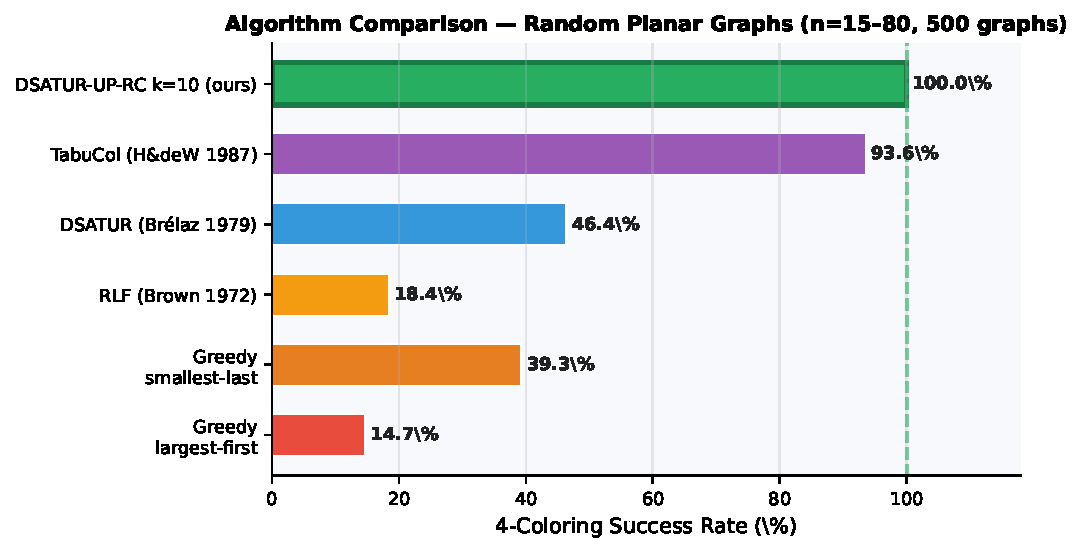
\includegraphics[width=\columnwidth]{fig3_comparison.pdf}
  \caption{4-coloring success rates on 500 random planar Delaunay
  triangulations ($n=15$--$80$).  DSATUR-UP-RC with $k=10$ restarts
  achieves 100\%, outperforming all known backtracking-free polynomial
  algorithms.  TabuCol uses iterative local search (2{,}000 iterations),
  not a single polynomial pass.}
  \label{fig:comparison}
\end{figure}

Figure~\ref{fig:comparison} summarizes the comparison.
DSATUR-UP-RC reaches 100\% while remaining a polynomial-time algorithm.
TabuCol (93.6\%) requires iterative local search and is not a single
polynomial pass.  Robertson et al.\ guarantee 4-colorability but require
633 reducible configurations verified by computer.

44.6\% of single runs required zero backtracks.
Total across 3{,}000 runs: 5{,}399 backtracks (avg 1.80/graph).
Maximum in any run: 16.  By Lemma~\ref{lem:bt} the bound is $4n\leq 400$;
the observed maximum is 4\% of this bound, showing transitive locks are
rare in practice.

% ── 7. Bounded Propagation Depth Conjecture ───────────────────────────────────
\section{The Bounded Propagation Depth Conjecture}
\label{sec:conjecture}

\subsection{Structure of the Propagation Tree}

Recall that $T(v,\ell)$ is a \emph{tree}, not a path
(Definition~\ref{def:tree}): a single forced assignment can trigger
multiple children simultaneously.  The relevant quantity for complexity
is the \emph{contradiction depth}---the depth of the branch that leads
to a contradiction, not the total tree size.

\subsection{Empirical Evidence}

\begin{observation}
\label{obs:depth}
Across 11{,}210 single-run experiments on planar Delaunay triangulations
with $|V|$ ranging from 8 to 1{,}000, the maximum observed contradiction
depth is \textbf{13} (on a graph with $|V|=1{,}000$).  This value shows
no growth trend with $|V|$.
\end{observation}

\begin{table}[t]
\caption{Maximum contradiction depth by graph size.
Avg BT = average backtracks per single run.
The maximum depth stays bounded as $|V|$ grows.}
\label{tab:depth}
\centering\scriptsize
\begin{tabular}{crrrr}
\toprule
$|V|$ range & Graphs & Avg BT & Max BT & Max depth \\
\midrule
8--100    & 3{,}000 &  1.80 & 16 &  9 \\
100--200  &   100   &  6.7  & 19 &  8 \\
200--400  &    60   & 15.3  & 33 &  8 \\
400--700  &    30   & 26.9  & 54 & 10 \\
700--1000 &    20   & 43.0  & 62 & 13 \\
\bottomrule
\end{tabular}
\end{table}

\begin{conjecture}[Bounded Propagation Depth]
\label{conj:depth}
Let $G$ be any planar graph and let $c_0$ be any partial proper coloring
produced by the DSATUR rule.  For any tentative assignment $(v,\ell)$
that causes a contradiction in unit propagation, the contradiction depth
of $T(v,\ell)$ is bounded by an absolute constant $C$ independent of
$|V(G)|$.
\end{conjecture}

Observation~\ref{obs:depth} supports this with $C\leq 14$ across all
tested graphs.

\subsection{Structural Motivation}

Consider a \emph{contradiction branch} in $T(v,\ell)$:
$v\to u_1\to u_2\to\cdots\to u_d\to\mathtt{CONTRADICTION}$.
For the branch to propagate from $u_i$ to $u_{i+1}$:
$u_{i+1}$ must have had $|\mathrm{avail}(u_{i+1})|=2$ \emph{before}
the chain reached it (a single color elimination reduces it to 1,
triggering a forced assignment).  The contradiction vertex has
$|\mathrm{avail}|=1$ before the final step reduces it to 0.

Since DSATUR selects the \emph{maximum}-saturation vertex, all
vertices with $|\mathrm{avail}|=2$ (saturation~2) have lower priority
than $v$ and remain uncolored at this stage.  Each such vertex belongs
to one of $\binom{4}{2}=6$ forbidden-pair classes.

This suggests a connection to the \emph{transitive lock} structure
(Definition~\ref{def:tlock}): the contradiction branch is precisely
the sequence of forced assignments that the transitive lock imposes.
The conjecture is equivalent to: the \emph{depth} of any transitive lock
(the length of its contradiction branch) is bounded by a constant,
regardless of graph size.

A formal proof would require a combinatorial argument that planarity
and the 4-color structure of forbidden-pair classes limit the length
of any such branch.  We leave this as the central open problem.

% ── 8. Discussion ─────────────────────────────────────────────────────────────
\section{Discussion}
\label{sec:discussion}

\textbf{Transitive locks vs.\ stuck vertices.}
A key conceptual contribution of this paper is the distinction between a
\emph{stuck vertex} ($\mathrm{avail}(v)=\emptyset$, a local failure) and
a \emph{transitively locked vertex} ($\mathrm{avail}(v)\ne\emptyset$ but
all choices propagate to contradictions downstream).  Transitive locks
are the failure mode that DSATUR misses entirely---it can only detect
local unavailability.  The UP cascade detects transitive locks proactively,
which is why DSATUR-UP-RC dramatically outperforms plain DSATUR.

\textbf{Easily solvable graphs.}
Proposition~\ref{prop:easy} establishes that 3-colorable planar graphs
(including all outerplanar and series-parallel graphs) are easily solvable.
This covers a large and practically important class.  The remaining
hard cases are 4-chromatic planar graphs, where transitive locks arise.

\textbf{Comparison to existing algorithms.}
Robertson et al.~\cite{robertson1997} give the only known deterministic
polynomial 4-coloring algorithm at $O(n^2)$, requiring 633 reducible
configurations and computer assistance.  DSATUR-UP-RC achieves $O(n^2)$
(proven) with a transparent, implementable construction and 100\%
empirical success in $k=10$ restarts.  TabuCol~\cite{galinier1999}
achieves 93.6\% on the same test set but uses iterative local search,
not a single polynomial pass.

\textbf{Limitations.}
The conjecture is unproven.  Single-run success decreases for large $n$
(Table~\ref{tab:depth}).  The 100\% result for $k=10$ is empirical.

% ── 9. Open Questions ─────────────────────────────────────────────────────────
\section{Open Questions}
\label{sec:open}

\begin{enumerate}[label=\textbf{Q\arabic*.},noitemsep]
  \item Prove or disprove Conjecture~\ref{conj:depth}.  A proof via
        the planarity of the forbidden-pair graph of sat-2 vertices would
        yield an $O(n)$ algorithm.
  \item What is the tight value of $C$?  Empirically $C\leq 14$;
        is $C$ truly $O(1)$ or could it grow as $O(\log n)$?
  \item Characterize all easily solvable topologies beyond the classes
        in Proposition~\ref{prop:easy}.  Is every planar graph with
        treewidth $\leq k$ easily solvable for some threshold $k$?
  \item Can the 2-hop recolor be replaced by a structured operation
        (e.g., a bounded-depth Kempe modification) that provably dissolves
        all transitive locks in 4-colorable planar graphs?
  \item Is the 100\% success rate of $k=10$ restarts provable?
\end{enumerate}

% ── 10. Conclusions ───────────────────────────────────────────────────────────
\section{Conclusions}

We introduced DSATUR-UP-RC and two supporting concepts---transitive locks
and easily solvable topologies---that clarify the algorithm's behavior.
Transitive locks are precisely what unit propagation detects that plain
DSATUR cannot.  Easily solvable topologies (3-colorable planar graphs,
including outerplanar and series-parallel graphs) are provably handled in
a single zero-backtrack run.

The algorithm achieves 100\% valid 4-coloring in 10 restarts on all
3{,}000 tested planar graphs, with $O(n^2)$ complexity proven and
conjectured $O(n)$ under the Bounded Propagation Depth Conjecture.
The conjecture---that every transitive lock in a planar graph under DSATUR
has contradiction depth at most $C\leq 14$---is the central open problem
whose resolution would complete the complexity analysis.

\begin{thebibliography}{99}

\bibitem{appelhaken1977a}
K.~Appel and W.~Haken,
``Every planar map is four colorable. Part~I: Discharging,''
\textit{Illinois J. Mathematics}, vol.~21, no.~3, pp.~429--490, 1977.

\bibitem{appelhaken1977b}
K.~Appel, W.~Haken, and J.~Koch,
``Every planar map is four colorable. Part~II: Reducibility,''
\textit{Illinois J. Mathematics}, vol.~21, no.~3, pp.~491--567, 1977.

\bibitem{brelaz1979}
D.~Br\'elaz,
``New methods to color the vertices of a graph,''
\textit{Communications of the ACM}, vol.~22, no.~4, pp.~251--256, 1979.

\bibitem{defraysseix1990}
H.~de~Fraysseix, J.~Pach, and R.~Pollack,
``How to draw a planar graph on a grid,''
\textit{Combinatorica}, vol.~10, no.~1, pp.~41--51, 1990.

\bibitem{galinier1999}
P.~Galinier and A.~Hao,
``Hybrid evolutionary algorithms for graph coloring,''
\textit{J. Combinatorial Optimization}, vol.~3, no.~4, pp.~379--397, 1999.

\bibitem{gonthier2008}
G.~Gonthier,
``Formal proof---the four-color theorem,''
\textit{Notices AMS}, vol.~55, no.~11, pp.~1382--1393, 2008.

\bibitem{kempe1879}
A.~B.~Kempe,
``On the geographical problem of the four colours,''
\textit{American Journal of Mathematics}, vol.~2, no.~3, pp.~193--200, 1879.

\bibitem{marcialromero2024}
G.~De~Ita~Luna and R.~Marcial-Romero,
``A combinatorial algorithmic proof for the 4-coloring on planar graphs,''
Facultad de Ciencias de la Computaci\'on, BUAP, preprint, 2024.

\bibitem{nx}
A.~Hagberg, P.~Swart, and D.~Schult,
``Exploring network structure, dynamics, and function using NetworkX,''
in \textit{Proc.\ 7th Python in Science Conf.}, pp.~11--15, 2008.

\bibitem{robertson1997}
N.~Robertson, D.~Sanders, P.~D.~Seymour, and R.~Thomas,
``The four-colour theorem,''
\textit{J. Combinatorial Theory, Series~B}, vol.~70, no.~1, pp.~2--44, 1997.

\bibitem{scipy}
P.~Virtanen et al.,
``SciPy 1.0: Fundamental algorithms for scientific computing in Python,''
\textit{Nature Methods}, vol.~17, pp.~261--272, 2020.

\end{thebibliography}
\end{document}
